% Created 2013-12-20 金 04:52
\documentclass[12pt]{jsarticle}
\usepackage[dvipdfmx]{graphicx}
\usepackage{comment}
%\usepackage{setspace}
%%\date{\today}
%\title{}
\textheight = 25truecm
\textwidth = 18truecm
\topmargin = -1.5truecm
\oddsidemargin = -1truecm
\evensidemargin = -1truecm
\marginparwidth = -1truecm
\def\theenumii{\Alph{enumii}}
\def\theenumiii{\alph{enumiii}}
\def\labelenumi{(\theenumi)}
\def\labelenumiii{(\theenumiii)}
%\setstretch{0.9}
\setlength\intextsep{0pt}
\setlength\textfloatsep{0pt}

\newcommand{\insertfigurecontents}[5][1]{
  \includegraphics[clip,width=#1\columnwidth]{\figdir/#3.\figext}
  \caption{#4}\ecaption{#5}\label{#2}
}

\newcommand{\insertfigure}[5][0.9]{
  \begin{figure}[tb]
    \begin{center}
      \insertfigurecontents[#1]{#2}{#3}{#4}{#5}
    \end{center}
  \end{figure}
}

\newcommand{\insertwidefigure}[5][0.9]{
  \begin{figure*}[tb]
    \begin{center}
      \insertfigurecontents[#1]{#2}{#3}{#4}{#5}
    \end{center}
  \end{figure*}
}
\begin{document}

%\maketitle
%\tableofcontents

\begin{center}
%%%%%%%%%%%%%%%%%%%%%%%%%%%%%%%%%%%%%%%
%%%タイトル                         %%%
%%%%%%%%%%%%%%%%%%%%%%%%%%%%%%%%%%%%%%%
{\LARGE 2015年度前期研究計画(藤田)(修正版)}
\end{center}

\begin{flushright}
  2015/4/20\\
  藤田将輝
\end{flushright}
%%%%%%%%%%%%%%%%%%1章%%%%%%%%%%%%%%%%%%%
\section{はじめに}
前回提出した2015年度前期研究計画(藤田)には,
研究テーマと,SwoPP2015の原稿締め切りが記載されていなかった.
また,今後の課題について誤った認識をしていた.
このため,本資料ではこれらの情報を加えた2015年度前期研究計画(藤田)の
修正版を示す.
\section{前回の研究計画との差異}
前回の研究計画との差異は以下の3つである.
\begin{enumerate}
    \item 研究テーマを記載していなかったため,研究テーマを
        記載した.
    \item SwoPP2015の原稿締め切りを記載していなかったため,
        SwoPP2015の原稿締め切りを記載した.
    \item パケットの受信を完了した後の課題について,
        NICドライバの受信処理時間を比較するとしていたが,
        これは誤りである.
        実際の課題としては,本環境によって実現できる通信量と
        本物のNICの通信量を比較し,評価することである.
\end{enumerate}
\section{研究テーマ}
\begin{description}
    \item[(題目)]Mintオペレーティングシステムを用いたNICドライバの
        割り込みデバッグ手法の実現
    \item[(概要)]
        OSの機能の中で,割り込み処理は,割り込みがいつ発生するかがわからないため,
        再現性の低さからデバッグが困難である.
        割り込み処理のデバッグの方法として,VMを用いたものがある.
        これはVM上で2つのOSを走行させ,一方のOSから他方のOSへ任意のタイミングで
        割り込みを発生させることにより,バグを再現し,デバッグを支援するものである.
        しかし,VMを用いたデバッグ手法ではVMとハイパーバイザ間の処理の遷移に伴う処理負荷が発
        生する.このため,一定間隔で発生する割り込みや短い間隔で発生するバグの
        ように処理負荷が影響する割り込み処理のデバッグが困難である.
        そこで,Mintを用いたOSのデバッグ手法が提案されている.Mintは1台の計
        算機上で複数のOSが計算機資源を分割占有して走行できる.本研究では,Mint
        において,NICによる割り込みを任意に挿入できる環境を実現する.具体的に
        は,割り込み元OSからNICドライバが割り込み処理をするパケットを共有メモ
        リに格納し,割り込み元OSが占有しているコアから割り込み先のOSが占有して
        いるコアへIPIを送信することにより,割り込みハンドラが動作し,NICドライ
        バが共有メモリからパケットを取得することで割り込み処理を発生させるもの
        である.これにより,NICドライバの割り込みにより発生するバグを再現し,
        デバッグを支援することができる.
\end{description}
\section{課題一覧}
藤田の
課題について以下で説明する.
\begin{description}
    \item[(大課題1)]Mintを用いたデバッグ手法の提案\\
        OSのデバッグを行う際に,特に困難であるのが,割り込み処理に関する
        デバッグである.割り込み処理は非同期な処理であり,いつ発生するかが
        予想できない.そこで,Mintを用いて,デバッグ支援OSとデバッグ対象OS
        を動作させ,任意のタイミングで割り込み処理を発生させる環境を
        構築し,デバッグを支援する.今回のデバッグ対象はNICドライバの
        パケット受信割り込み処理としている.
        現在は,受信割り込み処理の発生までを完了しているが,
        パケットの受信が未完了である.
        これを完了させた後,本環境で再現したNICの通信量と,本物のNICの通信量とを
        比較し,評価する.
        GbitEtherと比較し,GbitEtherよりも多くの通信量を実現できれば有用であると言える.
\end{description}
\section{今後の予定}
今後の予定について,図\ref{fig:plan}に示し,以下で説明する.
%\insertwidefigure[0.75]{plan}{fig/fig1}{2015年度前期研究計画}{Plan\_of\_research\_2015}
\begin{figure}[t]
    \begin{center}
    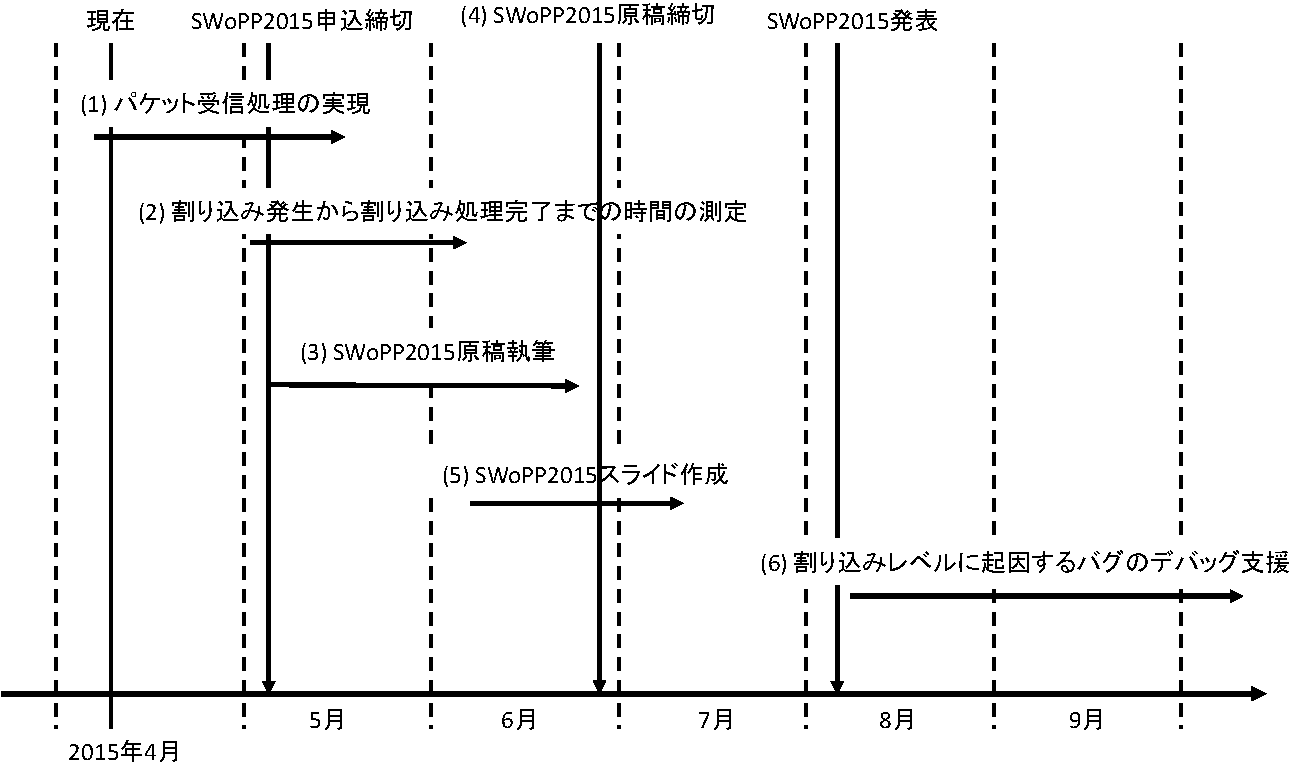
\includegraphics[clip,scale=0.65]{fig/fig1.pdf}
    \caption{2015年度前期研究計画}
    \label{fig:plan}
\end{center}
\end{figure}
\begin{enumerate}
    \item パケット受信処理の実現(2015年5月中旬)\\
        Etherフレームの構造を擬似したものを作成し,処理させる.
        パケットの種類はUDPとする.
    \item 本環境における,単位時間あたりの通信量の測定\\
        本環境において,単位時間あたりに受信できるパケットの量を
        測定し,本物のNICを用いた場合の通信量と比較する.
    \item SWoPP2015原稿執筆(2015年6月下旬)
    \item SWoPP2015原稿締め切り(2015年6月末)
    \item SWoPP2015の発表スライド作成(2015年7月上旬)
    \item 割り込みレベルに起因するバグのデバッグ支援(未定)\\
        割り込みレベルに起因するバグについて調査し,Mintを用いて,
        調査したバグを再現する.
\end{enumerate}
\section{学会情報}
\begin{enumerate}
    \item 2015年並列/分散/協調処理に関する『別府』サマー・ワークショップ (SWoPP2015)
        \begin{description}
            \item[開催期間:]平成27年8月4日(火)〜8月6日(木)
            \item[開催場所:] ビーコンプラザ 別府国際コンベンションセンター (大分県別府) 
            \item[原稿締め切り:]未定(6月末)
        \end{description}

\end{enumerate}
\section{おわりに}
本資料では,2015年度前期における藤田の研究計画を示した.
\end{document}


